%Correct the file name.
%X: book number
%Y: part number
%ZZZ: page number in three digits. So page 3 would be 003.

\documentclass[11pt]{amsbook}

\usepackage{booktabs}
\usepackage{mathtools}
\usepackage{amsmath}
\usepackage{amssymb}
\usepackage{arydshln}
\usepackage{../HBSuerDemir}	% ------------------------

\begin{document}

% ++++++++++++++++++++++++++++++++++++++
\hPage{b2p1/092}
% ++++++++++++++++++++++++++++++++++++++

Example. find the inverses of the matrices

$ a) A=\begin{bmatrix}
2 & 1 & 1 \\
1 & -2 & -1 \\
1 & 1 & 2
\end{bmatrix}$
$ b) B=\begin{bmatrix}
2 & 3 \\
6 & 9
\end{bmatrix}$

Solution.

$
\lvert A \enspace I \rvert = 
\left[\begin{array}{ccc|ccc}
2 & 1 & 1  & 1 & 0 & 0 \\
1 & -2 & -1 & 0 & 1 & 0 \\
1 & 1 & 2 & 0 & 0 & 1
\end{array}\right]
$
\newline

\begin{tabular}{ll}
$\thicksim\left[\begin{array}{ccc|ccc}
2 & 1 & 1  & 1 & 0 & 0 \\
1 & -2 & -1 & 0 & 1 & 0 \\
1 & 1 & 2 & 0 & 0 & 1
\end{array}\right]\begin{array}{ll} 
\downarrow & -2 \\ 
\multicolumn{2}{l}{\leftarrow} \\
\\\end{array}$
&
$\thicksim\left[\begin{array}{ccc|ccc}
2 & 1 & 1  & 0 & 1 & 0 \\
0 & 5 & 3 & 1 & -2 & 0 \\
1 & 1 & 2 & 0 & 0 & 1
\end{array}\right]
\begin{array}{cc} 
\Bigg\downarrow & -1 \\ 
\multicolumn{2}{l}{\leftarrow}\\ 
\\\end{array}$

\\

$\thicksim\left[\begin{array}{ccc|ccc}
2 & 1 & 1  & 1 & 0 & 0 \\
0 & 5 & 3 & 1 & -2 & 0 \\
0 & 3 & 3 & 0 & -1 & 1
\end{array}\right]
\begin{array}{c}\\ \\ \frac{1}{3} \\\end{array}$
&
$\thicksim\left[\begin{array}{ccc|ccc}
2 & 1 & 1  & 1 & 0 & 0 \\
0 & 5 & 3 & 1 & -2 & 0 \\
0 & 1 & 1 & 0 & -\frac{1}{3} & \frac{1}{3}
\end{array}\right]
\begin{array}{cc}
\\ \downarrow & -\frac{1}{5} 
\\ \multicolumn{2}{l}{\leftarrow}
\\\end{array}$

\\

$\thicksim\left[\begin{array}{ccc|ccc}
2 & 1 & 1  & 1 & 0 & 0 \\
0 & 5 & 3 & 1 & -2 & 0 \\
0 & 0 & \frac{2}{5} & -\frac{1}{5} & \frac{1}{15} & \frac{1}{3}
\end{array}\right]
\begin{array}{c} \\ (1/5) \\ (5/2) \\\end{array}$
&
$\thicksim\left[\begin{array}{ccc|ccc}
1 & -2 & -1  & 0 & 1 & 0 \\
0 & 1 & \frac{3}{5} & \frac{1}{5} & -\frac{2}{5} & 0 \\
0 & 0 & 1 & -\frac{1}{2} & \frac{1}{6} & \frac{5}{6}
\end{array}\right]
\begin{array}{cc} 
\multicolumn{2}{l}{\leftarrow} \\ 
\uparrow & 2 \\ \\\end{array}$

\\

$\thicksim\left[\begin{array}{ccc|ccc}
1 &  & \frac{1}{5}  & \frac{2}{5} & \frac{1}{5} & 0 \\
0 & 1 & \frac{3}{5} & \frac{1}{5} & -\frac{2}{5} & 0 \\
0 & 0 & 1 & -\frac{1}{2} & \frac{1}{6} & \frac{5}{6}
\end{array}\right]
\begin{array}{c}\\ \\ -\frac{1}{5}\\\end{array}$
&
$\thicksim\left[\begin{array}{ccc|ccc}
1 &  & 0  & \frac{1}{2} & \frac{1}{6} & -\frac{1}{6} \\
0 & 1 & \frac{3}{5} & \frac{1}{5} & -\frac{2}{5} & 0 \\
0 & 0 & 1 & -\frac{1}{2} & \frac{1}{6} & \frac{5}{6}
\end{array}\right]
\begin{array}{cc} 
\\ 
\multicolumn{2}{l}{\leftarrow} \\ 
\uparrow & -\frac{3}{5} \\\end{array}$

\\

\multicolumn{2}{l}
{
	$\thicksim\left[\begin{array}{ccc|ccc}
	1 &  & 0  & \frac{1}{2} & \frac{1}{6} & -\frac{1}{6} \\
	0 & 1 & 0 & \frac{1}{2} & -\frac{1}{2} & -\frac{1}{2} \\
	0 & 0 & 1 & -\frac{1}{2} & \frac{1}{6} & \frac{5}{6}
	\end{array}\right]\Rightarrow\enspace
	A^{-1} =
	\left[\begin{array}{ccc}
	\frac{1}{2} & \frac{1}{6} & -\frac{1}{6} \\
	\frac{1}{2} & -\frac{1}{2} & -\frac{1}{2} \\
	-\frac{1}{2} & \frac{1}{6} & \frac{5}{6}
	\end{array}\right]$
	}

\end{tabular}

% =======================================================
\end{document}  

%==== templates ====

%==== environments ====

%\begin{figure}[htb]
%	\centering
%	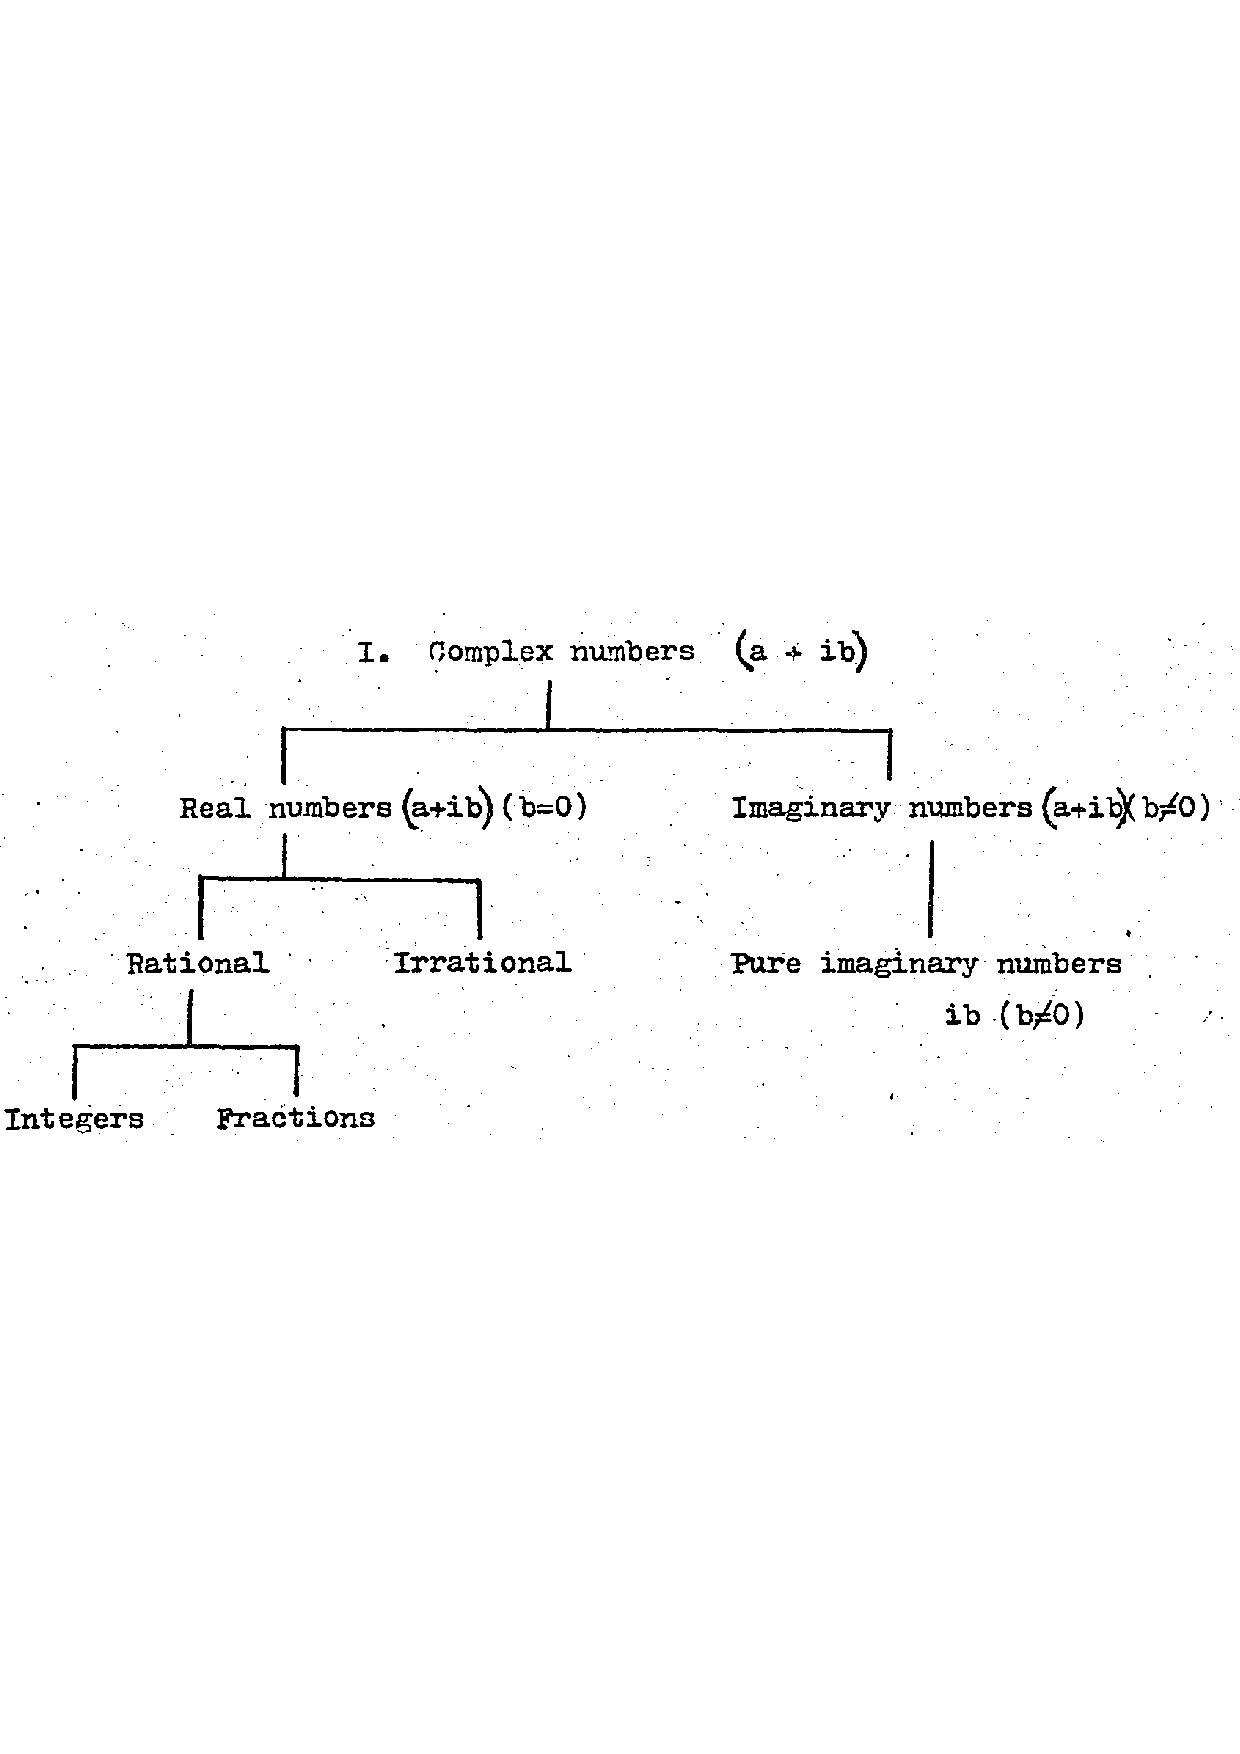
\includegraphics[width=0.9\textwidth]{images/SD-1-1p15A}
%	\caption{Classification of complex numbers}
%	\label{fig:classificationOfComplexNumbersA}
%\end{figure}

%\begin{center}
%\begin{tabular}{cc}
%\end{tabular}
%\end{center}

%\begin{exmp}
%\begin{hSolution}
%\end{hSolution}
%\end{exmp}

%\begin{hEnumerateAlpha}
%\end{hEnumerateAlpha}

%\begin{hEnumerateRoman}
%\end{hEnumerateRoman}

%$
%\begin{bmatrix}
%\end{bmatrix}
%$

%\frac{aaaa}{bbb}
%\frac{a_{n}}{b_{n}}
%\left( aaaa \right)
%\Longrightarrow

%\begin{multicols}{2}
%	bb
%\columnbreak
%	aa
%\end{multicols}
